\documentclass{standalone}
\usepackage{tikz}
\usetikzlibrary{patterns, positioning}
\usepackage[sfdefault]{ClearSans} %% option 'sfdefault' activates Clear Sans as the default text font
\usepackage[T1]{fontenc}

\begin{document}
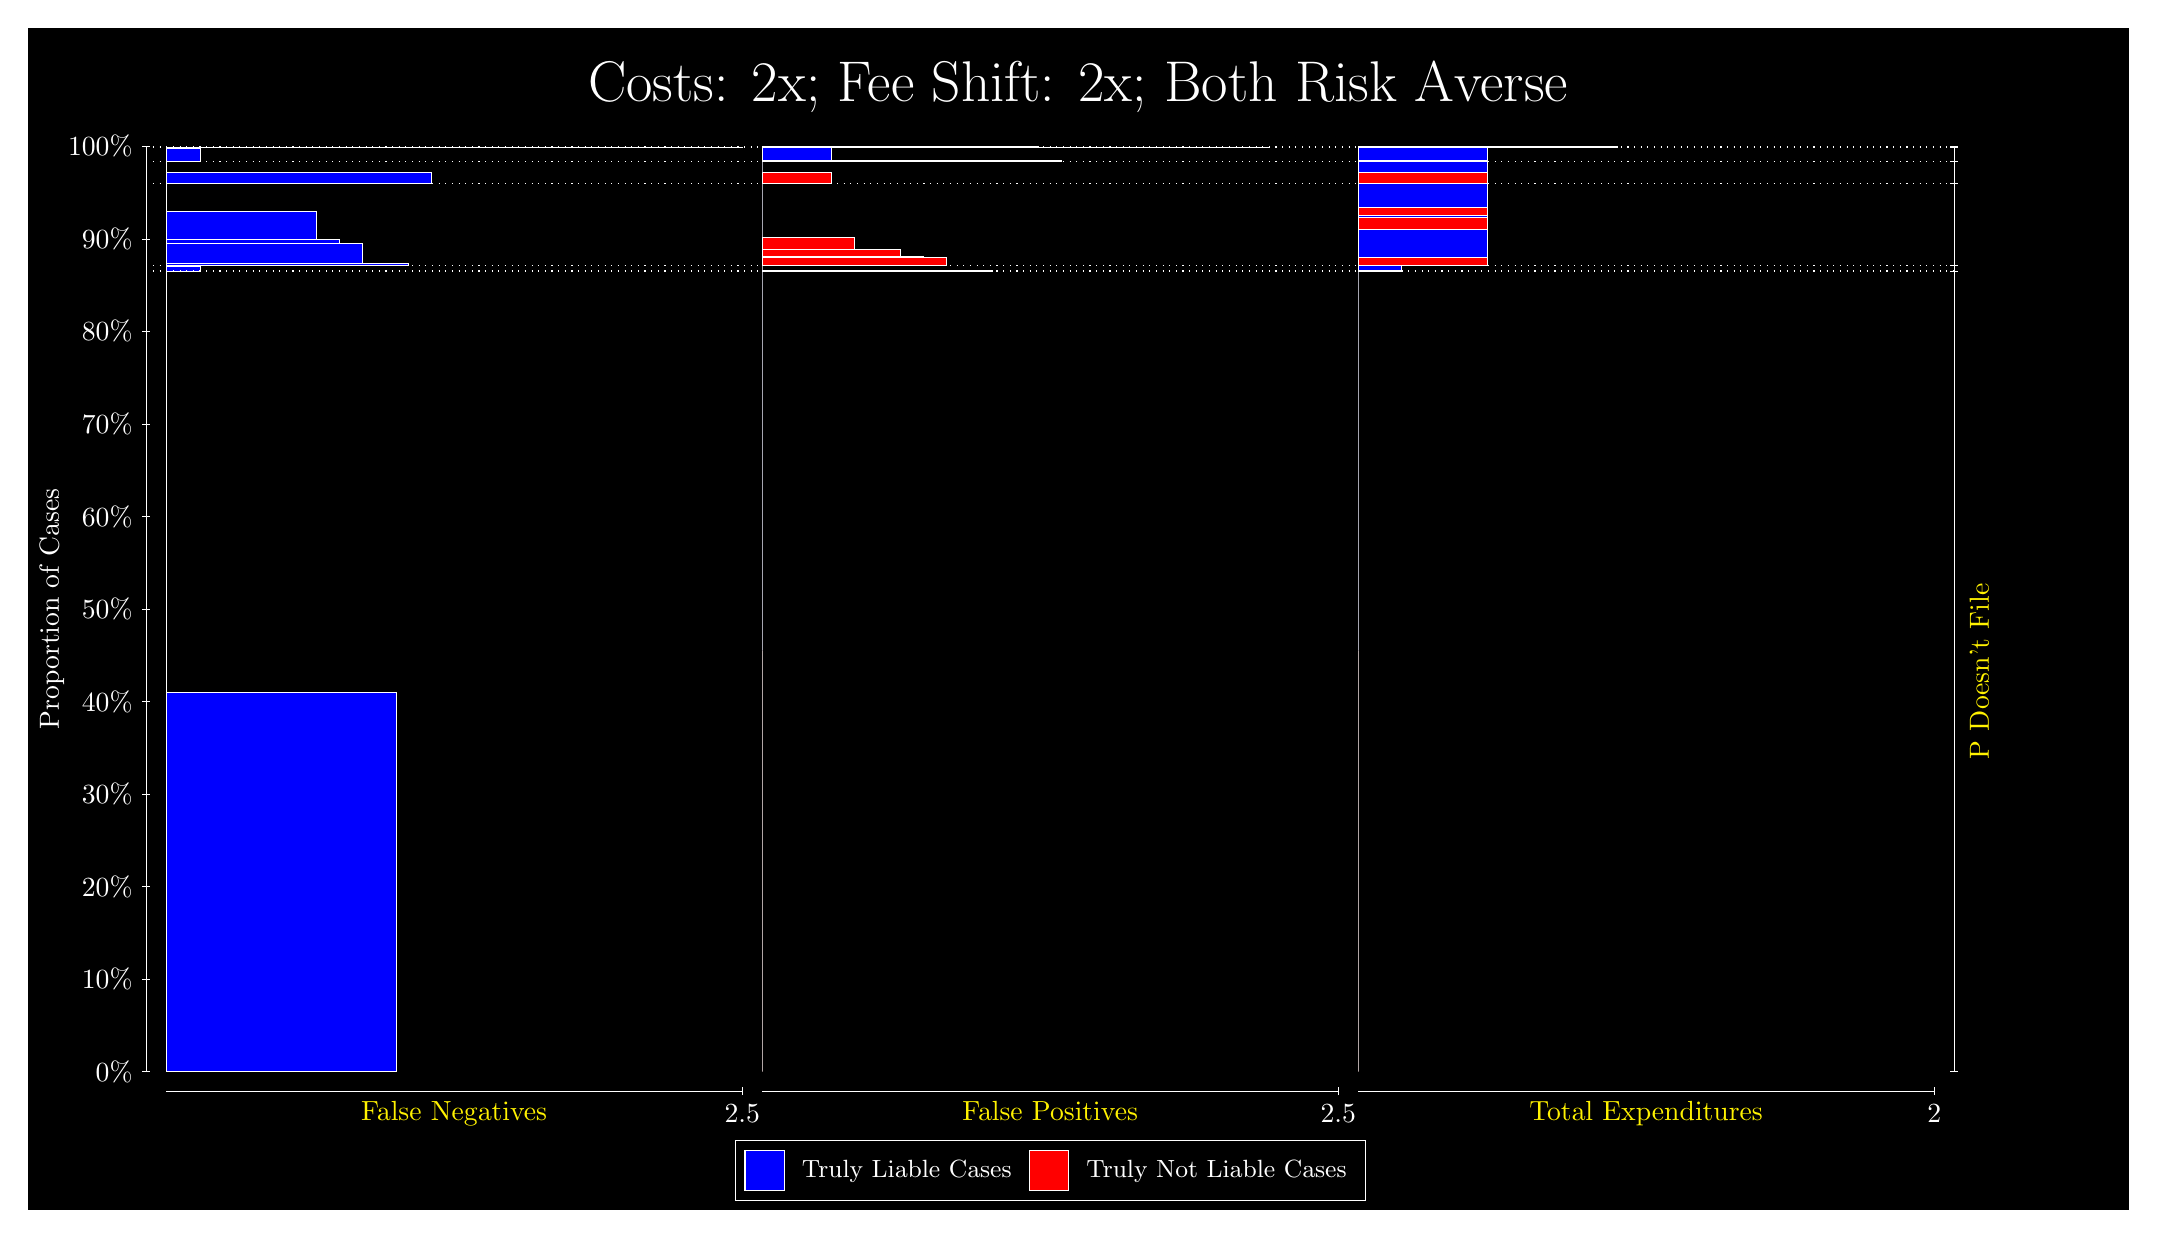
\begin{tikzpicture}
\draw[fill=black] (0,0) rectangle (26.667,15);
\draw[text=white] (0,13.5) rectangle (26.667,15) node[midway] {\huge Costs: 2x; Fee Shift: 2x; Both Risk Averse};
\draw[white, very thin] (1.5,1.75) -- (1.5,13.5);
\node[rotate=90, text=white, anchor=center] at (0.3, 7.625) {Proportion of Cases};
\draw[white, very thin] (1.45,1.75) -- (1.55,1.75);
\node[text=white, anchor=east] at (1.45, 1.75) {0\%};
\draw[white, very thin] (1.45,2.925) -- (1.55,2.925);
\node[text=white, anchor=east] at (1.45, 2.925) {10\%};
\draw[white, very thin] (1.45,4.1) -- (1.55,4.1);
\node[text=white, anchor=east] at (1.45, 4.1) {20\%};
\draw[white, very thin] (1.45,5.275) -- (1.55,5.275);
\node[text=white, anchor=east] at (1.45, 5.275) {30\%};
\draw[white, very thin] (1.45,6.45) -- (1.55,6.45);
\node[text=white, anchor=east] at (1.45, 6.45) {40\%};
\draw[white, very thin] (1.45,7.625) -- (1.55,7.625);
\node[text=white, anchor=east] at (1.45, 7.625) {50\%};
\draw[white, very thin] (1.45,8.8) -- (1.55,8.8);
\node[text=white, anchor=east] at (1.45, 8.8) {60\%};
\draw[white, very thin] (1.45,9.975) -- (1.55,9.975);
\node[text=white, anchor=east] at (1.45, 9.975) {70\%};
\draw[white, very thin] (1.45,11.15) -- (1.55,11.15);
\node[text=white, anchor=east] at (1.45, 11.15) {80\%};
\draw[white, very thin] (1.45,12.325) -- (1.55,12.325);
\node[text=white, anchor=east] at (1.45, 12.325) {90\%};
\draw[white, very thin] (1.45,13.5) -- (1.55,13.5);
\node[text=white, anchor=east] at (1.45, 13.5) {100\%};

\draw[white, very thin] (24.457,1.75) -- (24.457,13.5);
\draw[white, very thin] (24.407,1.75) -- (24.507,1.75);
\node[anchor=west] at (24.407, 1.75) {};
\draw[white, very thin] (24.407,11.917) -- (24.507,11.917);
\node[anchor=west] at (24.407, 11.917) {};
\draw[white, very thin] (24.407,11.989) -- (24.507,11.989);
\node[anchor=west] at (24.407, 11.989) {};
\draw[white, very thin] (24.407,13.031) -- (24.507,13.031);
\node[anchor=west] at (24.407, 13.031) {};
\draw[white, very thin] (24.407,13.306) -- (24.507,13.306);
\node[anchor=west] at (24.407, 13.306) {};
\draw[white, very thin] (24.407,13.489) -- (24.507,13.489);
\node[anchor=west] at (24.407, 13.489) {};
\draw[white, very thin] (24.407,13.492) -- (24.507,13.492);
\node[anchor=west] at (24.407, 13.492) {};
\draw[white, very thin] (24.407,13.5) -- (24.507,13.5);
\node[anchor=west] at (24.407, 13.5) {};

\draw[white, very thin, fill=blue] (1.75,1.75) rectangle (4.6775,6.5671);
\draw[white, very thin, fill=red] (1.75,6.5671) rectangle (1.75,11.917);
\draw[white, very thin, fill=blue] (1.75,11.917) rectangle (2.1891,11.982);
\draw[white, very thin, fill=red] (1.75,11.982) rectangle (1.75,11.989);
\draw[white, very thin, fill=blue] (1.75,11.989) rectangle (4.8239,12.013);
\draw[white, very thin, fill=blue] (1.75,12.013) rectangle (4.2384,12.275);
\draw[white, very thin, fill=blue] (1.75,12.275) rectangle (3.9457,12.323);
\draw[white, very thin, fill=blue] (1.75,12.323) rectangle (3.6529,12.67);
\draw[white, very thin, fill=red] (1.75,12.67) rectangle (1.75,13.031);
\draw[white, very thin, fill=blue] (1.75,13.031) rectangle (5.1167,13.17);
\draw[white, very thin, fill=red] (1.75,13.17) rectangle (1.75,13.306);
\draw[white, very thin, fill=blue] (1.75,13.306) rectangle (2.1891,13.472);
\draw[white, very thin, fill=red] (1.75,13.472) rectangle (1.75,13.489);
\draw[white, very thin, fill=blue] (1.75,13.489) rectangle (9.0689,13.491);
\draw[white, very thin, fill=red] (1.75,13.491) rectangle (1.75,13.492);
\draw[white, very thin, fill=red] (1.75,13.492) rectangle (1.75,13.494);
\draw[white, very thin, fill=blue] (1.75,13.494) rectangle (1.75,13.5);
\draw[white, very thin, fill=red] (9.3189,1.75) rectangle (9.3189,7.1001);
\draw[white, very thin, fill=blue] (9.3189,7.1001) rectangle (9.3189,11.917);
\draw[white, very thin, fill=red] (9.3189,11.917) rectangle (12.246,11.925);
\draw[white, very thin, fill=blue] (9.3189,11.925) rectangle (9.3189,11.989);
\draw[white, very thin, fill=red] (9.3189,11.989) rectangle (11.661,12.096);
\draw[white, very thin, fill=red] (9.3189,12.096) rectangle (11.368,12.1);
\draw[white, very thin, fill=red] (9.3189,12.1) rectangle (11.075,12.195);
\draw[white, very thin, fill=red] (9.3189,12.195) rectangle (10.49,12.35);
\draw[white, very thin, fill=blue] (9.3189,12.35) rectangle (9.3189,13.031);
\draw[white, very thin, fill=red] (9.3189,13.031) rectangle (10.197,13.167);
\draw[white, very thin, fill=blue] (9.3189,13.167) rectangle (9.3189,13.306);
\draw[white, very thin, fill=red] (9.3189,13.306) rectangle (13.125,13.324);
\draw[white, very thin, fill=blue] (9.3189,13.324) rectangle (10.197,13.489);
\draw[white, very thin, fill=red] (9.3189,13.489) rectangle (9.3189,13.491);
\draw[white, very thin, fill=blue] (9.3189,13.491) rectangle (9.3189,13.492);
\draw[white, very thin, fill=red] (9.3189,13.492) rectangle (15.759,13.494);
\draw[white, very thin, fill=blue] (9.3189,13.494) rectangle (12.832,13.5);
\draw[white, very thin, fill=red] (16.888,1.75) rectangle (16.888,7.1001);
\draw[white, very thin, fill=blue] (16.888,7.1001) rectangle (16.888,11.917);
\draw[white, very thin, fill=red] (16.888,11.917) rectangle (17.437,11.925);
\draw[white, very thin, fill=blue] (16.888,11.925) rectangle (17.437,11.989);
\draw[white, very thin, fill=red] (16.888,11.989) rectangle (18.534,12.096);
\draw[white, very thin, fill=blue] (16.888,12.096) rectangle (18.534,12.443);
\draw[white, very thin, fill=red] (16.888,12.443) rectangle (18.534,12.597);
\draw[white, very thin, fill=blue] (16.888,12.597) rectangle (18.534,12.622);
\draw[white, very thin, fill=red] (16.888,12.622) rectangle (18.534,12.721);
\draw[white, very thin, fill=blue] (16.888,12.721) rectangle (18.534,13.031);
\draw[white, very thin, fill=red] (16.888,13.031) rectangle (18.534,13.167);
\draw[white, very thin, fill=blue] (16.888,13.167) rectangle (18.534,13.306);
\draw[white, very thin, fill=red] (16.888,13.306) rectangle (18.534,13.324);
\draw[white, very thin, fill=blue] (16.888,13.324) rectangle (18.534,13.489);
\draw[white, very thin, fill=red] (16.888,13.489) rectangle (20.181,13.491);
\draw[white, very thin, fill=blue] (16.888,13.491) rectangle (20.181,13.492);
\draw[white, very thin, fill=red] (16.888,13.492) rectangle (20.181,13.494);
\draw[white, very thin, fill=blue] (16.888,13.494) rectangle (20.181,13.5);
\draw[white, dotted] (1.5,11.917) -- (24.457,11.917);
\draw[white, dotted] (1.5,11.989) -- (24.457,11.989);
\draw[white, dotted] (1.5,13.031) -- (24.457,13.031);
\draw[white, dotted] (1.5,13.306) -- (24.457,13.306);
\draw[white, dotted] (1.5,13.489) -- (24.457,13.489);
\draw[white, dotted] (1.5,13.492) -- (24.457,13.492);
\draw[white, very thin] (1.75,1.5) -- (9.0689,1.5);
\node[text=yellow, anchor=north] at (5.4094, 1.5) {False Negatives};
\draw[white, very thin] (9.0689,1.45) -- (9.0689,1.55);
\node[text=white, anchor=north] at (9.0689, 1.45) {2.5};

\draw[white, very thin] (9.3189,1.5) -- (16.638,1.5);
\node[text=yellow, anchor=north] at (12.978, 1.5) {False Positives};
\draw[white, very thin] (16.638,1.45) -- (16.638,1.55);
\node[text=white, anchor=north] at (16.638, 1.45) {2.5};

\draw[white, very thin] (16.888,1.5) -- (24.207,1.5);
\node[text=yellow, anchor=north] at (20.547, 1.5) {Total Expenditures};
\draw[white, very thin] (24.207,1.45) -- (24.207,1.55);
\node[text=white, anchor=north] at (24.207, 1.45) {2};

\node[text=yellow, centered, rotate=90] at (24.777, 6.8336) {P Doesn't File};







\draw (12.978300999999998,1.5) node[draw=none] (baseCoordinate) {};
\begin{scope}[align=center]
        \matrix[scale=0.5, draw=white, below=0.5cm of baseCoordinate, nodes={draw}, column sep=0.1cm]{
            \node[rectangle, draw, minimum width=0.5cm, minimum height=0.5cm, fill=blue] {}; &
            \node[draw=none, font=\small, text=white] (B) {Truly Liable Cases}; &
            \node[rectangle, draw, minimum width=0.5cm, minimum height=0.5cm, fill=red] {}; &
            \node[draw=none, font=\small, text=white] (B) {Truly Not Liable Cases}; \\
            };
\end{scope}

\end{tikzpicture}
\end{document}